\documentclass{article}
 
%Russian-specific packages
%--------------------------------------
\usepackage[T2A]{fontenc}
\usepackage[utf8]{inputenc}
\usepackage[russian]{babel}
%--------------------------------------
 
%Hyphenation rules
%--------------------------------------
\usepackage{hyphenat}
\hyphenation{ма-те-ма-ти-ка вос-ста-нав-ли-вать}
%--------------------------------------

\title{Приватность в блокчейне}
\author{Михаил Койпиш }
\date{Декабрь 2018}

\usepackage{natbib}
\usepackage{graphicx}

\begin{document}

\maketitle

\section{Введение}
There is a theory which states that if ever anyone discovers exactly what the Universe is for and why it is here, it will instantly disappear and be replaced by something even more bizarre and inexplicable.
There is another theory which states that this has already happened.

\begin{figure}[h!]
\centering
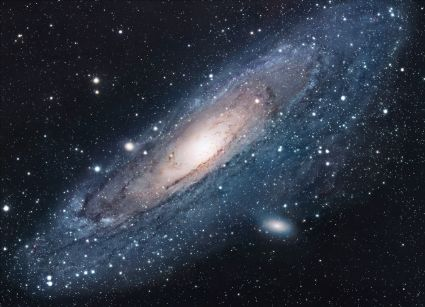
\includegraphics[scale=1.7]{universe}
\caption{The Universe}
\label{fig:universe}
\end{figure}

\section{Конфиденциальные транзакции в Bitcoin}
ывавадовыафываываывафывфываываыфвафываывафывафываываывафываываывафываыва    фыавфываывафываываыва
sdfdf
ывавыавыаывафы
фываываываывафыва
asdfghjkl
фываываываываываывавыа
фывапролд
ываываываыва
\bibliographystyle{plain}
\bibliography{references}
\end{document}
